\section{Slučajevi upotrebe}

Slučaj upotrebe je specifikacija skupa akcija koje vrši sistem. Koristi se da
precizira ponašanje sistema.

\subsection{Prodaja}

\begin{figure}[ht]
\centering
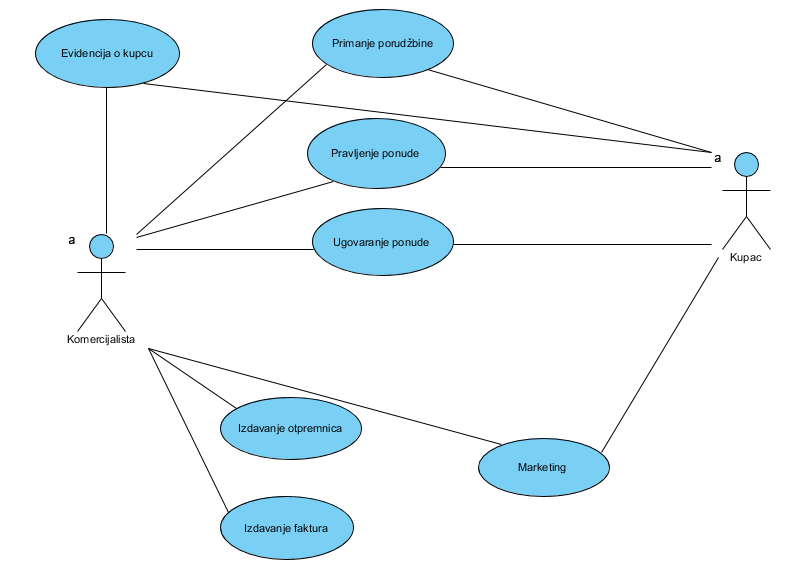
\includegraphics[width=120mm]{slike/useCaseProdaja.png}%
\caption{Dijagram slučajeva upotrebe vezanih za prodaju}
\end{figure}

\clearpage

\subsubsection{Evidencija o kupcu}

\textbf{Opis:}

Evidentiranje kupca kao pravnog lica i kontakt osobe iz te firme.
\newline
\textbf{Akteri:}

Kupac - daje potrebne informacije

Komercijalista - traži od kupca potrebne informacije
\newline
\textbf{Preduslov:}

Ostvaren je kontakt sa kupcem ili se planira saradnja.
\newline
\textbf{Postuslov:}

Uspešno uneti podaci u bazu.
\newline
\textbf{Glavni tok:}

1. Komercijalista ulazi u deo programa koji se bavi evidencijom.

2. Prikazuje se tabela sa svim unešenim kupcima. 

Zatim slede koraci u zavisnosti od potrebnog.

\textit{Čitanje}

1. Klikom na konretnog kupca prikazuju mu se detaljnije 	informacije o kupcu tj. firmi, između koji je i lista zaposlenih u toj firmi o kojima imamo podatke.

\textit{Dodavanje}

1. Opcija ”Dodaj novog kupca” otvara formu za unos, unosi podatke o firmi iz APR(Agencija za privredne registre) koji su dostupni sa interneta.

2. U okviru ove postoji dodatne opcija za ”Dodaj novog zaposlenog”, otvara formu za unos podataka o zaposleno iz konkretne firme. Uglavnom će to biti komercijlisti sa kojim samo u kontaktu.

\textit{Ažuriranje}

1. Opcija ”Izmene” postoji pored svakog postojećeg kupca. Pomoću koje menjamo postojeće podatke.

2. Klikom opcije ”Izmena” pored postojećih zaposlenih menjamo podatke o njima.

\textit{Brisanje}

1. Opcija ”Obriši” postoji pored svakog postojećeg kupca. Pomoću koje brišemo postojeće podatke.

2. Klikom opcije ”Obriši” pored postojećih zaposlenih brišemo podatke o njima.

\textbf{Napomena:}
Izmena i brisanje zaposlenih u nekoj firmi mogu se izvoditi nezavisno od izmena firme.
Svaka firma ima jedinstveni matični i poreski broj, pa nije moguće više puta unošenje iste firme.

\clearpage

\subsubsection{Marketing}

\textbf{Opis:}

Plasiranje reklamnog materijala u postizanju većeg plasmana robe.
\newline
\textbf{Akteri:}

Kupac - prima reklamni promotivni materijal

Komercijalista - brine da su kupci informisani o najnovijim ponudama
\newline
\textbf{Preduslov:}

Kupci su evidentirani i postoje u bazi podataka.
\newline
\textbf{Postuslov:}

Kupac prima reklamni materijal.
\newline
\textbf{Glavni tok:}

1. Komercijalista ulazi u deo programa koji se bavi evidencijom.

2. Prikazuje se tabela sa svim unešenim kupcima. 

3. Klikom na konretnog kupca prikazuju mu se detaljnije informacije o kupcu.

4. Proverava informaciju o poslednjem slanju reklamnog materijala ka konkretnom kupcu.

5. Šalje se reklamni materijal.

6. Komercijalista ažurira datum slanja.

\textbf{Napomena:}
Veoma je bitno da se ne šalje svakodnevno materijal istom kupcu, čime bi se on osetio uvređenim. Nije dobro ni zapostaviti kupca i uopšte mu ne slati materijal.

\clearpage

\subsubsection{Primanje porudžbina}

\textbf{Opis:}

Kupac naručuje robu, koju komercijalista zavodi u sistem kao porudžbinu.
\newline
\textbf{Akteri:}

Kupac - naručuje potrebne lekove

Komercijalista - sastavlja porudžbinu u skladu sa željama kupca i mogućnostima isporuke
\newline
\textbf{Preduslov:}

Kupac je evidentiran i postoji u bazi podataka.
\newline
\textbf{Postuslov:}

Porudžbina uneta u bazu.
\newline
\textbf{Glavni tok:}

1. Kupac kontaktira komercijalistu i šalje mu porudžbinu putem mejla. 

2. Komercijalista ulazi u deo programa za prodaju, podsekcija za porudžbine

3. Bira opciju da kreira novu porudžbinu, čime mu izlazi forma za popunjavanje porudžbine.

4. Opcija sačuvaj , skladišti podatke u bazu.
\newline
\textbf{Alternativni tok:}

2.1  Eventualno se dogovara oko supstitucija za neki lek(da uzme neki drugi lek sa istim dejstvima umesto navedenog)
\newline
\textbf{Izlazni dokument:}

Porudžbina sačuvana u bazi i vezana za kupca.
\newline
\textbf{Napomena:}

Porudžbina se sastoji od lekova i željenih količina. Kao i do kada mu treba isporuka. Porudžbina nekad zahteva pojašnjenje kupcu oko dejstava pojedinih lekova.

\clearpage

\subsubsection{Pravljenje ponude}

\textbf{Opis:}

Komercijalista od primljene porudžbine sastavlja ponudu.
\newline
\textbf{Akteri:}

Komercijalista - sastavlja ponudu prema porudžbini kupca

Menadžer - može dati nekom kupcu promotivne cene

\textbf{Preduslov:}

Porudžbina evidentirana i postoji u bazi podataka.
\newline
\textbf{Postuslov:}

Ponuda uneta u bazu.
\newline
\textbf{Glavni tok:}

1. Komercijalista pronalazi u bazi porudžbinu.

2. Komercijalista pristupa delu programa za prodaja, podsekcija ponuda.

3. Opcija "dodaj" otvara formu o kojoj se sastavlja ponuda.

4. Opcija sačuvaj , skladišti podatke u bazu.

5. Imejlom dostavlja kupcu napravljenu ponudu.

\textbf{Alternativni tok:}
1.1 Menadžer konkretnom kupcu daje odredjene popuste.

3.1 Kupac se javlja da izmeni porudžbinu.

3.2 Komercijalista u ažurira porudžbinu i ponudu.

\textbf{Izlazni dokument:}

Ponuda sačuvana u bazi i vezana za kupca.

\textbf{Napomena:}
U nekim ponudama može menadžer učestvovati i ponuditi popust određenom kupcu, u cilju privlačenja kupca i buduće bolje saradnje.
Forma nove ponude pored auto-completa za imena lekova,radi konzistentnosti, ima i automatsku uvoz cene za odgovarajući lek. Kao i generisanje konacne sume, dobijene na osnovu cena lekova i količina poručenih.

\clearpage

\begin{figure}[ht]
\centering
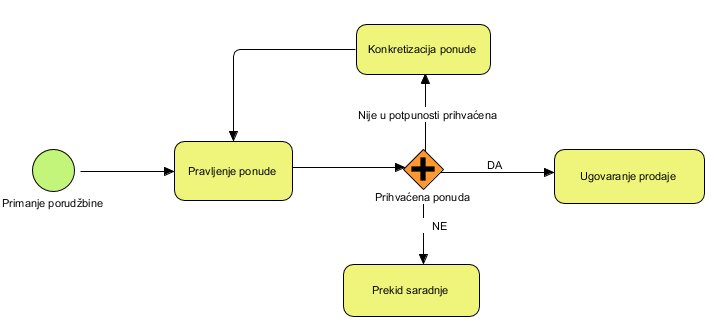
\includegraphics[width=120mm]{slike/BPMN-pravljenje-ponude.png}%
\caption{BPMN dijagram za ugovaranja ponude.}
\end{figure}

\subsubsection{Ugovaranje ponude}

\textbf{Opis:}

Ugovaranje ponude sa kupcem, u cilju ostvarivanja prodaje, na obostrano zadovoljstvo.
\newline
\textbf{Akteri:}

Kupac - izjašnjava se oko pristigle ponude

Komercijalista - može da menja ponudu na zahtev kupca

\textbf{Preduslov:}

Ponuda uneta i postoji u bazi podataka.
\newline
\textbf{Postuslov:}

Obe strane zadovoljne poslom, kupovina će se izvršiti.
\newline
\textbf{Glavni tok:}

1. Kupac izjašnjava oko ponude.

2. Kupac pristaje na ponudu.
\newline
\textbf{Alternativni tok:}

1.1 Kupac nije upotpunosti zadovoljan ponudom.

1.2 Komercijalista u dogovoru sa kupcem ažurira ponudu (Konretizacija ponude).

1.3 Komercijalista pravi novu poboljšanu ponudu.
\newline
Drugi alternativni tok.

2. Kupcu ne odgovara ponuda.

3. Trenutna saradnja se završava.

\clearpage

\subsubsection{Izdavanje otpremnica}

\textbf{Opis:}

Komercijalista izdaje otpremnicu koju čuva u bazi, za koju je kasnije zadužen magacin. Bitna je za odvajanje robe za isporuku.
\newline
\textbf{Akteri:}

Komercijalista - pravi otpremnicu na osnovu ugovorene ponude

\textbf{Preduslov:}

Ponuda postoji u bazi i ponude je ugovorena sa kupcem.
\newline
\textbf{Postuslov:}

Gotova otpremnica, koja je potrebna magacinu.
\newline
\textbf{Glavni tok:}

1. Komercijalista pristupa delu programa za prodaju, podsekcija otpremnice.

2. Opcija "dodaj" otvara formu o kojoj se pravi otpremnica.

3. Opcija sačuvaj , skladišti podatke u bazu.
\newline

\textbf{Izlazni dokument:}

Otpremnica za koju je kasnije zadužen magacin.

\textbf{Napomena:}
Otpremnica sadrži vrste artikala i količinu , ne i novčanu protivvrednost.

\subsubsection{Izdavanje fakture}

\textbf{Opis:}

Komercijalista izdaje fakturu koju čuva u bazi, za koju je kasnije zadužen knjigovođa. Bitna je za plaćanje robe.
\newline
\textbf{Akteri:}

Komercijalista - pravi fakturu na osnovu otpremnice

\textbf{Preduslov:}

U bazi postoji ugovorena ponuda i optremnica za tu ponudu.
\newline
\textbf{Postuslov:}

Gotova faktura, koja je potrebna knjigovodstvu.
\newline
\textbf{Glavni tok:}

1. Komercijalista pristupa delu programa za prodaju, podsekcija fakture.

2. Opcija "dodaj" otvara formu o kojoj se pravi faktura.

3. Opcija sačuvaj , skladišti podatke u bazu.
\newline

\textbf{Izlazni dokument:}

Faktura za koju je kasnije zaduženo knjigovodstvo.

\textbf{Napomena:}
Faktura sadrži vrste artikala i količinu kao i otpremnica , zajedno sa novčanom protivvrednosti.